% !TEX TS-program = pdflatex
%\RequirePackage{lineno}
\documentclass[aps,prc,onecolumn,floatfix,showpacs,preprintnumbers,amsmath,amssymb,superscriptaddress]{revtex4-1}
\usepackage{hyperref}
\usepackage{latexsym}
\usepackage{verbatim}
\usepackage{graphics}
\usepackage{caption}
\usepackage{subfigure}
\usepackage{amsmath}
\captionsetup{justification=centerlast,font=small,margin=0.5cm}
\usepackage{setspace}
\usepackage{graphicx,amsmath,color}% Include figure files
\providecommand{\Journal}[4] {#1 {\bf #2}, #3 (#4)}
\providecommand{\EPJC}{Eur. Phys. J. C }
\providecommand{\NCA}{Nuovo Cimento }
\providecommand{\NIM}{Nucl. Instr. Methods }
\providecommand{\NIMA}{Nucl. Instr. Meth. A }
\providecommand{\NPA}{Nucl. Phys. A }
\providecommand{\NPB}{Nucl. Phys. B }
\providecommand{\NHPA}{Nucl. Hadr. Phys. A }
\providecommand{\PLB}{Phys. Lett. B }
\providecommand{\PR}{Phys. Rev. }
\providecommand{\PRL}{Phys. Rev. Lett. }
\providecommand{\PRC}{Phys. Rev. C }
\providecommand{\PRD}{Phys. Rev. D }
\providecommand{\RMP}{Rev. Mod. Phys. }
\providecommand{\ZPC}{Z. Phys. C }
\providecommand{\qqb}{$q\bar{q}$~}
\newcommand{\bff}{{}}

\definecolor{lightred}{rgb}{1,0.5,0.5}
\definecolor{lightgreen}{rgb}{0.5,1,0.5}
\definecolor{darkgreen}{rgb}{0.5,0.9,0.5}
\def\piz{\pi^{0}}
\def\pizT{$\pi^{0} \ $}
\def\epemT{$ e^+e^-  $}
\def\epem{e^+e^-}
\begin{document}
\preprint{}


\title{Photoproduction of $\pi^0$ on Hydrogen Target with CLAS}

%To be submitted to Phys. Rev. Lett.\\
%\bf -- DRAFT -- VERSION 1.1\\
%\bf \today}

\newcommand*{\ODU}{Old Dominion University, Norfolk, VA 23529, USA}
%\newcommand*{\FZI}{J"\ulich, Germany}
\newcommand*{\BOCHUM}{Institut f\"ur Kernphysik, Forschungszentrum 
	J\"ulich 52424, J\"ulich, Germany; JARA-FAME (Forces and 
	Matter Experiments), Forschungszentrum J\"ulich and RWTH 
	Aachen University, 52056 Aachen, Germany}
\newcommand*{\PNPI}{Petersburg Nuclear Physics
	Institute, Gatchina, St.\ Petersburg 188300, Russia}
\newcommand*{\KYUNGPOOK} {Kyungpook National University, 702-701, Daegu, 
	Republic of Korea}
\newcommand*{\INR}{Institute for Nuclear Research, 117312, Moscow, Russia}
\newcommand*{\GWU}{The George Washington University, Washington, DC 20052}
\newcommand*{\CUA}{Catholic University of America, Washington, DC 20064} 
\newcommand*{\JLAB}{Thomas Jefferson National Accelerator Facility, Newport 
	News, VA 23606}
\newcommand*{\UVA}{University of Virginia, Charlottesville, VA 22904, USA}
\newcommand*{\CMU}{Carnegie Mellon University, Pittsburg, PA 15213, USA}

\newcommand*{\ANL}{Argonne National Laboratory, Argonne, IL 60439, USA}
\newcommand*{\ASU}{Arizona State University, Tempe, AZ 85287, USA}
\newcommand*{\CSUDH}{California State University, Dominguez Hills, Carson, 
	CA 90747, USA}
\newcommand*{\CANISIUS}{Canisius College, Buffalo, NY, USA}
\newcommand*{\SACLAY}{CEA, Centre de Saclay, Irfu/Service de Physique 
	Nucl\'eaire, 91191 Gif-sur-Yvette, France}
\newcommand*{\CNU}{Christopher Newport University, Newport News, VA 23606, 
	USA}
\newcommand*{\UCONN}{University of Connecticut, Storrs, CO 06269, USA}
\newcommand*{\EDINBURGH}{University of Edinburgh, Edinburgh EH9 3JZ, United 
	Kingdom}
\newcommand*{\FU}{Fairfield University, Fairfield, CT 06824, USA}
\newcommand*{\FIU}{Florida International University, Miami, FL 33199, USA}
\newcommand*{\FSU}{Florida State University, Tallahassee, FL 32306, USA}
\newcommand*{\GWUI}{The George Washington University, Washington, DC 20052, 
	USA}
\newcommand*{\ISU}{Idaho State University, Pocatello, Idaho 83209, USA}
\newcommand*{\INFNFE}{INFN, Sezione di Ferrara, 44100 Ferrara, Italy}
\newcommand*{\INFNFR}{INFN, Laboratori Nazionali di Frascati, 00044 Frascati, 
	Italy}
\newcommand*{\INFNGE}{INFN, Sezione di Genova, 16146 Genova, Italy}
\newcommand*{\INFNRO}{INFN, Sezione di Roma Tor Vergata, 00133 Rome, Italy}
\newcommand*{\ORSAY}{Institut de Physique Nucl\'eaire ORSAY, Orsay, France}
\newcommand*{\ITEP}{Institute of Theoretical and Experimental Physics, Moscow, 
	117259, Russia}
\newcommand*{\JMU}{James Madison University, Harrisonburg, VA 22807, USA}
\newcommand*{\KNU}{Kyungpook National University, Daegu 702-701, Republic of 
	Korea}
\newcommand*{\LPSC}{LPSC, Universite Joseph Fourier, CNRS/IN2P3, INPG, Grenoble, 
	France

}
\newcommand*{\UNH}{University of New Hampshire, Durham, New Hampshire 03824, 
	USA}
\newcommand*{\NSU}{Norfolk State University, Norfolk, VA 23504, USA}
\newcommand*{\OHIOU}{Ohio University, Athens, Ohio  45701, USA}
\newcommand*{\RPI}{Rensselaer Polytechnic Institute, Troy, NY 12180, USA}
\newcommand*{\ROMAII}{Universita' di Roma Tor Vergata, 00133 Rome Italy}
\newcommand*{\MSU}{Skobeltsyn Nuclear Physics Institute, 119899 Moscow, Russia}
\newcommand*{\SCAROLINA}{University of South Carolina, Columbia, South Carolina 
	29208, USA}
\newcommand*{\UNIONC}{Union College, Schenectady, NY 12308}
\newcommand*{\UTFSM}{Universidad T\'{e}cnica Federico Santa Mar\'{i}a, Casilla 
	110-V Valpara\'{i}so, Chile}
\newcommand*{\GLASGOW}{University of Glasgow, Glasgow G12 8QQ, United Kingdom}
\newcommand*{\VIRGINIA}{University of Virginia, Charlottesville, VA 22901, 
	USA}
\newcommand*{\WM}{College of William and Mary, Williamsburg, VA 23187, USA}
\newcommand*{\YEREVAN}{Yerevan Physics Institute, 375036 Yerevan, Armenia}
\newcommand*{\NOWCNU}{Christopher Newport University, Newport News, VA
	23606, USA}
\newcommand*{\NOWLANL}{Los Alamos National Laboratory, Los Alamos, NM 87544, 
	USA}
\newcommand*{\NOWMSU}{Skobeltsyn Nuclear Physics Institute, 119899 Moscow, 
	Russia}
\newcommand*{\NOWORSAY}{Institut de Physique Nucl\'eaire ORSAY, Orsay, France}
 %%%%%%%%%%%%%%% END OF Latex Macros for institute addresses  %%%%%%%%%%%%%%%%%%%%%%

\author {Michael~C.~Kunkel}
%\email{heghines@jlab.org}
%\affiliation{\ODU}
\altaffiliation[Now at ]{Forschungszentrum J\"ulich}%Lines break automatically or can be forced with \\
\author {Moskov~J.~Amaryan}
\thanks{Corresponding author.}
\email{mamaryan@odu.edu}
\affiliation{\ODU}
\author {Igor~I.~Strakovsky}
\affiliation{\GWU}
\author {James~Ritman}
\affiliation{\BOCHUM}

%\author {K.P. ~Adhikari} 
%\affiliation{\ODU}
%\author {D.~Adikaram} 
%\affiliation{\ODU}
%\author {M.~Aghasyan} 
%\affiliation{\INFNFR}
%\author {M.D.~Anderson} 
%\affiliation{\GLASGOW}
%\author {S. ~Anefalos~Pereira} 
%\affiliation{\INFNFR}
%\author {H.~Avakian} 
%\affiliation{\JLAB}
%\author {J.~Ball} 
%\affiliation{\SACLAY}
%\author {N.A.~Baltzell} 
%\affiliation{\ANL}
%\affiliation{\SCAROLINA}
%\author {M.~Battaglieri} 
%\affiliation{\INFNGE}
%\author {V.~Batourine} 
%\affiliation{\JLAB}
%\affiliation{\KNU}
%\author {I.~Bedlinskiy} 
%\affiliation{\ITEP}
%\author {R. P.~Bennett} 
%\affiliation{\ODU}
%\author {A.S.~Biselli} 
%\affiliation{\FU}
%\author {J.~Bono} 
%\affiliation{\FIU}
%\author {S.~Boiarinov} 
%\affiliation{\JLAB}
%\author {W.J.~Briscoe} 
%\affiliation{\GWUI}
%\author {W.K.~Brooks} 
%\affiliation{\UTFSM}
%\affiliation{\JLAB}
%\author {S.~B\"{u}ltmann} 
%\affiliation{\ODU}
%\author {V.D.~Burkert} 
%\affiliation{\JLAB}
%\author {D.S.~Carman} 
%\affiliation{\JLAB}
%\author {A.~Celentano} 
%\affiliation{\INFNGE}
%\author {S. ~Chandavar} 
%\affiliation{\OHIOU}
%\author {P.~Collins} 
%\affiliation{\CUA}
%\author {M.~Contalbrigo} 
%\affiliation{\INFNFE}
%\author {O. Cortes} 
%\affiliation{\ISU}
%\author {V.~Crede} 
%\affiliation{\FSU}
%\author {A.~D'Angelo} 
%\affiliation{\INFNRO}
%\affiliation{\ROMAII}
%\author {N.~Dashyan} 
%\affiliation{\YEREVAN}
%\author {R.~De~Vita} 
%\affiliation{\INFNGE}
%\author {E.~De~Sanctis} 
%\affiliation{\INFNFR}
%\author {A.~Deur} 
%\affiliation{\JLAB}
%\author {C.~Djalali} 
%\affiliation{\SCAROLINA}
%\author {D.~Doughty} 
%\affiliation{\CNU}
%\affiliation{\JLAB}
%\author {M.~Dugger} 
%\affiliation{\ASU}
%\author {R.~Dupre} 
%\affiliation{\ORSAY}
%\author {L.~El~Fassi} 
%\affiliation{\ANL}
%\author {P.~Eugenio} 
%\affiliation{\FSU}
%\author {G.~Fedotov} 
%\affiliation{\SCAROLINA}
%\affiliation{\MSU}
%\author {S.~Fegan} 
%\affiliation{\INFNGE}
%\author {R.~Fersch} 
%\altaffiliation[Current address:]{\NOWCNU}
%\affiliation{\WM}
%\author {J.A.~Fleming} 
%\affiliation{\EDINBURGH}
%\author {N.~Gevorgyan} 
%\affiliation{\YEREVAN}
%\author {K.L.~Giovanetti} 
%\affiliation{\JMU}
%\author {F.X.~Girod} 
%\affiliation{\JLAB}
%\affiliation{\SACLAY}
%\author {J.T.~Goetz} 
%\affiliation{\OHIOU}
%\author {W.~Gohn} 
%\affiliation{\UCONN}
%\author {E.~Golovatch} 
%\affiliation{\MSU}
%\author {R.W.~Gothe} 
%\affiliation{\SCAROLINA}
%\author {K.A.~Griffioen} 
%\affiliation{\WM}
%\author {M.~Guidal} 
%\affiliation{\ORSAY}
%\author {N.~Guler} 
%\altaffiliation[Current address:]{\NOWLANL}
%\affiliation{\ODU}
%\author {L.~Guo} 
%\affiliation{\FIU}
%\affiliation{\JLAB}
%\author {K.~Hafidi} 
%\affiliation{\ANL}
%\author {H.~Hakobyan} 
%\affiliation{\UTFSM}
%\affiliation{\YEREVAN}
%\author {C.~Hanretty} 
%\affiliation{\VIRGINIA}
%\affiliation{\FSU}
%\author {N.~Harrison} 
%\affiliation{\UCONN}
%\author {D.~Heddle} 
%\affiliation{\CNU}
%\affiliation{\JLAB}
%\author {K.~Hicks} 
%\affiliation{\OHIOU}
%\author {D.~Ho} 
%\affiliation{\CMU}
%\author {M.~Holtrop} 
%\affiliation{\UNH}
%\author {C.E.~Hyde} 
%\affiliation{\ODU}
%\author {Y.~Ilieva} 
%\affiliation{\SCAROLINA}
%\affiliation{\GWUI}
%\author {D.G.~Ireland} 
%\affiliation{\GLASGOW}
%\author {B.S.~Ishkhanov} 
%\affiliation{\MSU}
%\author {E.L.~Isupov} 
%\affiliation{\MSU}
%\author {H.S.~Jo} 
%\affiliation{\ORSAY}
%\author {K.~Joo} 
%\affiliation{\UCONN}
%\author {D.~Keller} 
%\affiliation{\VIRGINIA}
%\author {M.~Khandaker} 
%\affiliation{\NSU}
%\author {A.~Kim} 
%\affiliation{\KNU}
%\author {F.J.~Klein} 
%\affiliation{\CUA}
%\author {S.~Koirala} 
%\affiliation{\ODU}
%\author {A.~Kubarovsky} 
%\affiliation{\UCONN}
%\affiliation{\MSU}
%\author {V.~Kubarovsky} 
%\affiliation{\JLAB}
%\affiliation{\RPI}
%\author {S.E.~Kuhn} 
%\affiliation{\ODU}
%\author {S.V.~Kuleshov} 
%\affiliation{\UTFSM}
%\affiliation{\ITEP}
%\author {S.~Lewis} 
%\affiliation{\GLASGOW}
%\author {K.~Livingston} 
%\affiliation{\GLASGOW}
%\author {H.Y.~Lu} 
%\affiliation{\CMU}
%\affiliation{\SCAROLINA}
%\author {I .J .D.~MacGregor} 
%\affiliation{\GLASGOW}
%\author {D.~Martinez} 
%\affiliation{\ISU}
%\author {M.~Mayer} 
%\affiliation{\ODU}
%\author {B.~McKinnon} 
%\affiliation{\GLASGOW}
%\author {T.~Mineeva} 
%\affiliation{\UCONN}
%\author {M.~Mirazita} 
%\affiliation{\INFNFR}
%\author {V.~Mokeev} 
%\altaffiliation[Current address:]{\NOWMSU}
%\affiliation{\JLAB}
%\affiliation{\MSU}
%\author {R.A.~Montgomery} 
%\affiliation{\GLASGOW}
%\author {H.~Moutarde} 
%\affiliation{\SACLAY}
%\author {E.~Munevar} 
%\affiliation{\JLAB}
%\affiliation{\GWUI}
%\author {C. Munoz Camacho} 
%\affiliation{\ORSAY}
%\author {P.~Nadel-Turonski} 
%\affiliation{\JLAB}
%\author {R.~Nasseripour} 
%\affiliation{\JMU}
%\affiliation{\SCAROLINA}
%\author {S.~Niccolai} 
%\affiliation{\ORSAY}
%\author {I.~Niculescu} 
%\affiliation{\JMU}
%\author {M.~Osipenko} 
%\affiliation{\INFNGE}
%\author {A.I.~Ostrovidov} 
%\affiliation{\FSU}
%\author {L.L.~Pappalardo} 
%\affiliation{\INFNFE}
%\author {R.~Paremuzyan} 
%\altaffiliation[Current address:]{\NOWORSAY}
%\affiliation{\YEREVAN}
%\author {K.~Park} 
%\affiliation{\JLAB}
%\affiliation{\KNU}
%\author {S.~Park} 
%\affiliation{\FSU}
%\author {E.~Pasyuk} 
%\affiliation{\JLAB}
%\affiliation{\ASU}
%\author {E.~Phelps} 
%\affiliation{\SCAROLINA}
%\author {J.J.~Phillips} 
%\affiliation{\GLASGOW}
%\author {S.~Pisano} 
%\affiliation{\INFNFR}
%\author {O.~Pogorelko} 
%\affiliation{\ITEP}
%\author {S.~Pozdniakov} 
%\affiliation{\ITEP}
%\author {J.W.~Price} 
%\affiliation{\CSUDH}
%\author {D.~Protopopescu} 
%\affiliation{\GLASGOW}
%\author {A.J.R.~Puckett} 
%\affiliation{\JLAB}
%\author {D. ~Rimal} 
%\affiliation{\FIU}
%\author {M.~Ripani} 
%\affiliation{\INFNGE}
%\author {B.G.~Ritchie} 
%\affiliation{\ASU}
%\author {G.~Rosner} 
%\affiliation{\GLASGOW}
%\author {P.~Rossi} 
%\affiliation{\INFNFR}
%\affiliation{\JLAB}
%\author {F.~Sabati\'e} 
%\affiliation{\SACLAY}
%\author {M.S.~Saini} 
%\affiliation{\FSU}
%\author {C.~Salgado} 
%\affiliation{\NSU}
%\author {D.~Schott} 
%\affiliation{\GWUI}
%\author {R.A.~Schumacher} 
%\affiliation{\CMU}
%\author {E.~Seder} 
%\affiliation{\UCONN}
%\author {Y.G.~Sharabian} 
%\affiliation{\JLAB}
%\author {G.D.~Smith} 
%\affiliation{\GLASGOW}
%\author {D.I.~Sober} 
%\affiliation{\CUA}
%\author {D.~Sokhan} 
%\affiliation{\GLASGOW}
%\affiliation{\EDINBURGH}
%\author {S.~Stepanyan} 
%\affiliation{\JLAB}
%\author {P.~Stoler} 
%\affiliation{\RPI}
%\author {I.I.~Strakovsky} 
%\affiliation{\GWUI}
%\author {S.~Strauch} 
%\affiliation{\SCAROLINA}
%\affiliation{\GWUI}
%\author {W. ~Tang} 
%\affiliation{\OHIOU}
%\author {C.E.~Taylor} 
%\affiliation{\ISU}
%\author {Ye~Tian} 
%\affiliation{\SCAROLINA}
%\author {S.~Tkachenko} 
%\affiliation{\VIRGINIA}
%\affiliation{\ODU}
%\author {M.F.~Vineyard} 
%\affiliation{\UNIONC}
%\author {H.~Voskanyan} 
%\affiliation{\YEREVAN}
%\author {E.~Voutier} 
%\affiliation{\LPSC}
%\author {N.K.~Walford} 
%\affiliation{\CUA}
%\author {D.P.~Watts} 
%\affiliation{\EDINBURGH}
%\author {L.B.~Weinstein} 
%\affiliation{\ODU}
%\author {M.H.~Wood} 
%\affiliation{\CANISIUS}
%\affiliation{\SCAROLINA}
%\author {R.L.~Workman}
%\affiliation{\GWU}
%\author {N.~Zachariou} 
%\affiliation{\SCAROLINA}
%\author {L.~Zana} 
%\affiliation{\UNH}
%\author {J.~Zhang} 
%\affiliation{\JLAB}
%\author {Z.W.~Zhao} 
%\affiliation{\VIRGINIA}

%\include{odu_authors}
%\include{clas_authors}
%\date{\today  \\
%{\bf -- DRAFT -- VERSION 0.0.0}}
%%%%%%%%%%%%%%%%%%%%%%%%%%%%%%%%%%%%%%%%%%%%%%%%%%%%%%%%%%%%%%%%%%%%%%%%%%%%
%
\vskip 1.50in
\vskip 2in

%---------------------------------------------
\begin{abstract}
\centerline{\Large Abstract}
\vskip 0.2in
We report first high precision measurement of exclusive $\pi^0$ 
photoproduction cross section in Dalitz decay and conversion mode on 
hydrogen target in a wide kinematic range with CLAS 
setup at Thomas Jefferson National Accelerator Facility. 
Measurement is performed in the reaction $\gamma p\to 
pe^+e^-X(\gamma)$ using tagged photon beam spanning in 
energy interval, covered "resonance" and "Regge" regimes, 
$E = 1.25-5.55$~GeV. In the final state of the reaction, the particles $pe^+e^-$ 
are detected while the photon is not detected. $\pi^0$ is 
identified in the missing mass of proton.  This new data are quadrupled 
the world bremsstrahlung database above E = 2~GeV. Our 
data appear to favor Regge pole model while disfavor 
handbag one.
\end{abstract}
%---------------------------------------------

\pacs{12.38.Aw, 13.60.Rj, 14.20.-c, 25.20.Lj}
\maketitle

%---------------------------------------------
\textbf{Introduction:} In elementary particle physics involving 
energies less than 2.5~GeV in the c.m.~ total energy $W$ 
("resonance" regime), the study of lightest mesons ($\pi^0$ and 
$\eta$) in photoproduction has always been a complementary tool to 
elastic $\pi$N scattering. 
At high energies single pion photoproduction can be used to test predictions of Regge theory, in which recent calculations~\cite{JPAC} have shown to describe the presented data well. Furthermore, these measurements have shown that the differential cross section for single pion photoproduction at fixed c.m. angles, $\theta_{c.m.}$, of $70^{\circ}$, $90^{\circ}$ and $110^{\circ}$ seem to scale as $\frac{d\sigma}{dt} \sim s^{2-n}f(\theta_{c.m.})$, where $s$ and $t$ are the Mandelstam variables and $n$ is the total number of interacting elementary fields in the initial and final state of the reaction. This is predicted by the constituent counting rule~\cite{scaling1,scaling2} and exclusive measurements in $pp$ and  $\bar{p}p$ elastic scattering~\cite{scalingexp5, scalingexp7}, meson-baryon $M p$ reactions~\cite{scalingexp7}, and photoproduction $\gamma N$~\cite{scalingexp2, scalingexp3, scalingexp4, scalingexp6, scalingexp8, scalingexp9, scalingexp10, scalingexp11} agree well with this rule. 
%The complications introduced by the 
%spin 1 of the photon was a matter of algebra rather than 
%a matter of dynamics; this is not the case in the high-energy 
%domain. Because photoproduction involves three kind of different 
%masses and because the spin of particles are high enough, one 
%encounters both the problem of daughter trajectories and of 
%conspiracy relations. Therefore, this process and the associated 
%one of vector meson production are really very interesting at 
%the present. The possibility that the scattering amplitude for 
%photoproduction might be reggeized has not been cast in doubt 
%as Ader, Capdeville, and Salin noticed~\cite{Ader}. 
This experiment is a unique opportunity to bridge resonance and 
high-energy, in particular, "Regge", regimes and increases 
available database above resonance range by significant amount.

%---------------------------------------------------
%\textbf{Regge Pole Model:} 
The Regge pole amplitudes rely on already known Regge 
trajectories and coupling constants. The unitary cut amplitudes 
count on the independent description of the elementary 
photoproduction and meson re-scattering on-shell amplitudes.  
\color{red}{This approach is "parameter free". There is little degree of 
freedom left. One possibility is the relative sign between 
amplitudes.}\color{blue}{These 3 sentences has grammatical errors. The first sentence has no definitive subject, therefore ambiguous. The second sentence is not linked to any other sentence and therefore an incomplete sentence. The third sentence does not define the relation of "Possibility"} \color{black}The phase between the poles and the elastic neutral 
pion re-scattering is fixed by unitarity (for the absorptive 
part and consequently for the real part), but the relative 
phase of the amplitudes in the inelastic cuts is not 
determined by the cross section of the corresponding elementary 
reactions. A second possibility is a more accurate description 
of these elementary cross sections, but this is second order.  
The Regge pole and cut model for near forward higher energies 
above resonance regime $\pi^0$ photoproduction have been developed by 
Ader, Capdeville, and Salin~\cite{Ader}, Goldstein and 
Owens~\cite{Goldstein}, Laget~\cite{Laget}, Mathieu, Fox, and 
Szczepaniak~\cite{Mathieu}, Donnachie and 
Kalashnikova~\cite{Donnachie}, and many others.

%--------------------------------------------------
%\textbf{GPD-based Handbag Model:} 
The introduction of the handbag mechanism, developed by Kroll 
\textit{et al.}~\cite{Kroll}, has provided complimentary 
possibilities for the interpretation of hard exclusive 
reactions. In this approach, the reaction is factorized into 
two parts, one quark from the incoming and one from the 
outgoing nucleon participate in the hard sub-process, which is 
calculable using pQCD. While the soft part consists of all the 
other partons that are spectators and can be described in 
terms of GPDs~\cite{HM}. This approach was developed to 
understand the nature of the observation which the HERMES 
Collaboration made~\cite{Moskov}.

Previous bremsstrahlung measurements for $2~\leq E\leq 
18$~GeV (1964 -- 1979) gave 451 $d\sigma/d\Omega$s data points for 
$\gamma p\to p\pi^0$~\cite{brem}.  While recent tagged CLAS 
$g1c$ measurement contribution for $2~\leq E\leq 2.9$~GeV 
is limited to 164 $d\sigma/d\Omega$s~\cite{du07} data points.  Meanwhile, 
existing bremsstrahlung world data on photoproduction of neutral 
pions on proton target have very large systematic uncertaintes 
and do not have sufficient accuracy to perform comprehensive 
phenomenological analyses.

In this work, we provide a large set of cross sections from 
E = 1.275--5.425~MeV in laboratory photon energy, corresponding 
to a c.m. energy $W$ range of 1.81--3.33~GeV.  In this paper, 
we have therefore tried to confront the Regge pole and handbag 
phenomenology with the new CLAS experimental information on the 
$d\sigma/d\Omega(|t|)$ for the $\gamma p\to\pi^0p$ above 
"resonance" regime. As will be seen, this data set (it 
quadrupled the world bremsstrahlung database above E = 2~GeV) 
and previous CLAS $g1c$ tagged measurements~\cite{du07} 
greatly constrains the high energy phenomenology.

%----------------------------------------------------------
\textbf{Experiment:} Experiment is performed with CLAS setup 
at TJNAF using tagged photon beam produced by bremsstrahlung 
from 5.72~GeV electrons of CEBAF accelerator, impinged on 
liquid hydrogen target. 

The reaction of interest is 
photoproduction of neutral pions on hydrogen target $\gamma 
p\to p\pi^0$, where the neutral pions were detected via external conversion, 
$\pi^0 \rightarrow \gamma \gamma \rightarrow e^+e^-\gamma$, and subsequent 
Dalitz decay, $\pi^0 \rightarrow \gamma^* \gamma \rightarrow e^+e^-\gamma$. 
The final state contains three charged tracks, $p;e^+;e^-$, which allows to run experiment with high 
current, and which otherwise wouldn't have been possible 
with single prong charged track, due to trigger and data 
acquisition limitations.
%with subsequent Dalitz decay $\pi^0\to e^+e^-
%\gamma$ and external conversion mode, $\pi^0\to\gamma\gamma \to e^+e^-
%\gamma$ . Preference given to Dalitz decay mode of $\pi^0$ 
%with very small branching ratio of $\sim 1.2\%$ compared 
%main decay mode $\pi^0\to\gamma\gamma$ with branching ratio 
%$\sim 98.8\%$~\cite{PDG} is twofold. First, we wanted to 
%study $M_{e+e-}$ dependence of $\pi^0$ cross section. Then 
%secondly and most importantly in the Dalitz decay mode, final 
%state contains three charged tracks, contrary to $\gamma
%\gamma$ decay, which allows to run experiment with high 
%current, and which otherwise wouldn't have been possible 
%with single prong charged track, due to trigger and data 
%acquisition limitations.
%--------------------------------------------------
\begin{figure}[htb!]
\centerline{
        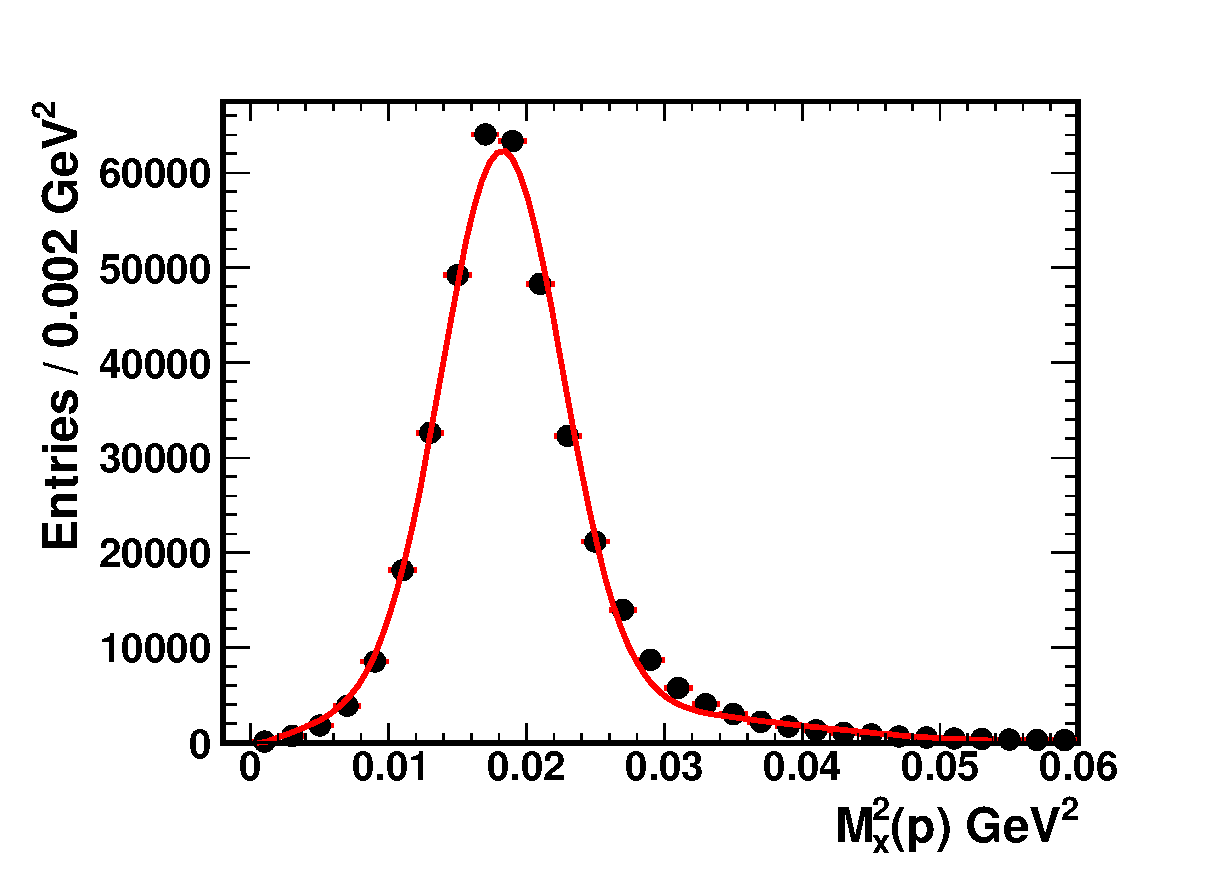
\includegraphics[width=3in, angle=0]{pi0_peak.eps}}

        \caption {(Color online) Peak of $\pi^0$ in the missing
                mass of proton for events with $pe^+e^-(\gamma)$
                in final state.} \label{fig:pi0_peak}
\end{figure}
%--------------------------------------------------

%----------------------------------------------------------
\textbf{Data analysis:} The missing mass of proton for events 
with $pe^+e^-(\gamma)$ in the final state is shown in 
Fig.~\ref{fig:pi0_peak}. The selected strategy of the analysis
of $g12$ data allowed to have negligible background.
The fit (shown by red solid line) performed with Gaussian plus 
3rd order polynomial function results in $M_{\pi^0}^2 = 
0.0182$~GeV$^2$ and Gaussian $\sigma=0.0043$~GeV$^2$.  

Lepton identification was based on conservation of mass. 
Once the data is skimmed for $p, \pi^+, \pi^-$, all particles that were 
$\pi^+$, $\pi^-$ were tentatively assigned to be electrons or positrons 
based on their charge (For details see~\cite{mkthesis}).
%This meant that the mass term of the particle's 
%4-vector was set to be the mass of an electron instead of that of a pion. 
%This technique works because the mass of the \pizT (0.135~GeV) is less 
%than the mass of $\pi^+$ or $\pi^-$ (0.139~GeV).
 After particle selection, standard g12 calibration, fiducial cuts ~\cite{g12note} and timing cuts were applied in the analysis.

The analysis employed three separate kinematic fitting hypotheses, 
4-C, 1-C and 2-C as well as a cut on the missing energy of the detected system.
 The 4-C fit used the $\gamma p \to p \pi^+ \pi^-$ 
channel to filter background from double charged pion production 
from single \pizT production. The 1-C fit was used for the topology 
of $\gamma p \rightarrow p e^+e^-(\gamma)$ to fit to a missing final 
state photon. The 2-C fit was used for the topology of $\gamma p \rightarrow p e^+e^-(\gamma)$ 
to fit to a missing final state photon but also to constrain the invariant 
mass of $e^+e^-(\gamma) = m_{\pi^0}^2$. The ``confidence levels'' for each constraint 
were consistent between g12 data and simulation. 

The remainder of the background was attributed to $\pi^+\pi^-$ events. To reduce the background further, a comparison of the missing mass squared off of the proton and the $p \epem$ missing energy of the system was performed. This comparison revealed that the majority of $\pi^+\pi^-$ background has missing energy less than 75~MeV. To eliminate this background all events with a missing energy less than ~75~MeV were removed.

Overall, angular independent systematic uncertainty varies between
9\% and 12\% as a function of photon beam energy. For the individual contributions of the systematic uncertainty see Tab.~\ref{tab:systematics}
\begin{table}[h!]
\begin{center}


\caption[Systematics]{\label{tab:systematics}Systematic errors used in $\frac{d\sigma}{d\cos\theta^{\pi^0}_{C.M.} d\phi}$ measurements \vspace{0.75mm}}

%\begin{tabular}{c|c}
\begin{tabular}{p{3.5cm} | p{4.75cm}}
\hline
Systematic & Error \\
\hline
Sector  & $ 0.0361 + 0.0065E_{\gamma}$ \\
Flux  & $ 0.06$ \\
Missing Energy Cut  & $0.02781$ \\
2-C Fit Pull Probability & $0.0219$ \\
1-C Fit Pull Probability  & $ 0.00216 + 0.01083E_{\gamma}$ \\
4-C Fit Pull Probability  & $0.00031$ \\ 
Target  & $0.005$ \\
Branching Ratio  & $0.0037$ \\
Fiducial Cut & $0.024$ \\
$z$-vertex Cut & $0.0041$ \\
%Total & $(0.0032 +0.00051E_{\gamma} +0.000184E_{\gamma}^2)^{\frac{1}{2}}$ \\
Total & $\sqrt{(5.7 +0.52E_{\gamma} +0.16E_{\gamma}^2)\cdot10^{-3}}$ \\
\hline \hline
\end{tabular}


\end{center}
\end{table}
\vspace{20pt}

%-----------------------------------------------------
\textbf{Results:} The new CLAS high statistical cross sections, 
obtained here, for $\gamma p\to\pi^0p$ are compared in 
Figs.~\ref{fig:scaling} and \ref{fig:t_data} with previous data 
from tagged JLab CLAS $g1c$~\cite{du07}, and bremsstrahlung DESY, 
Cambridge Electron Accelerator (CEA), and SLAC, and Electron 
Synchrotron at Cornell U~\cite{brem}. The overall agreement is 
good, specifically with the tagged CLAS $g1c$ measurements.
%----------------------------------------------------
\begin{figure}[htb!]
\centerline{
	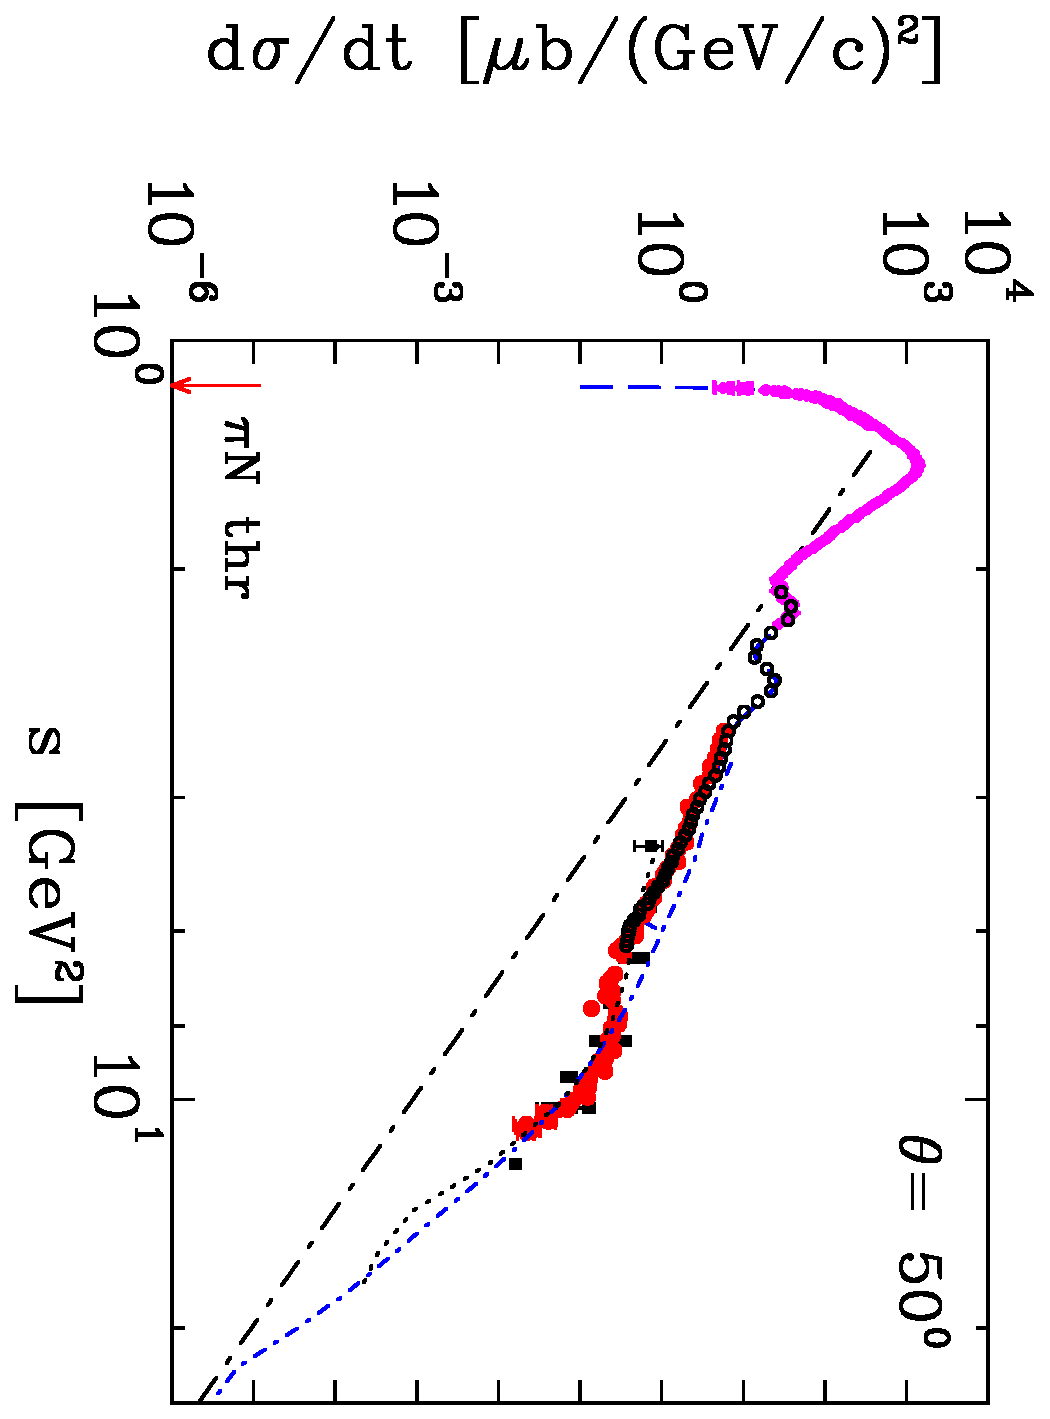
\includegraphics[height=0.4\textwidth, angle=90]{scale50.eps}\hfill
	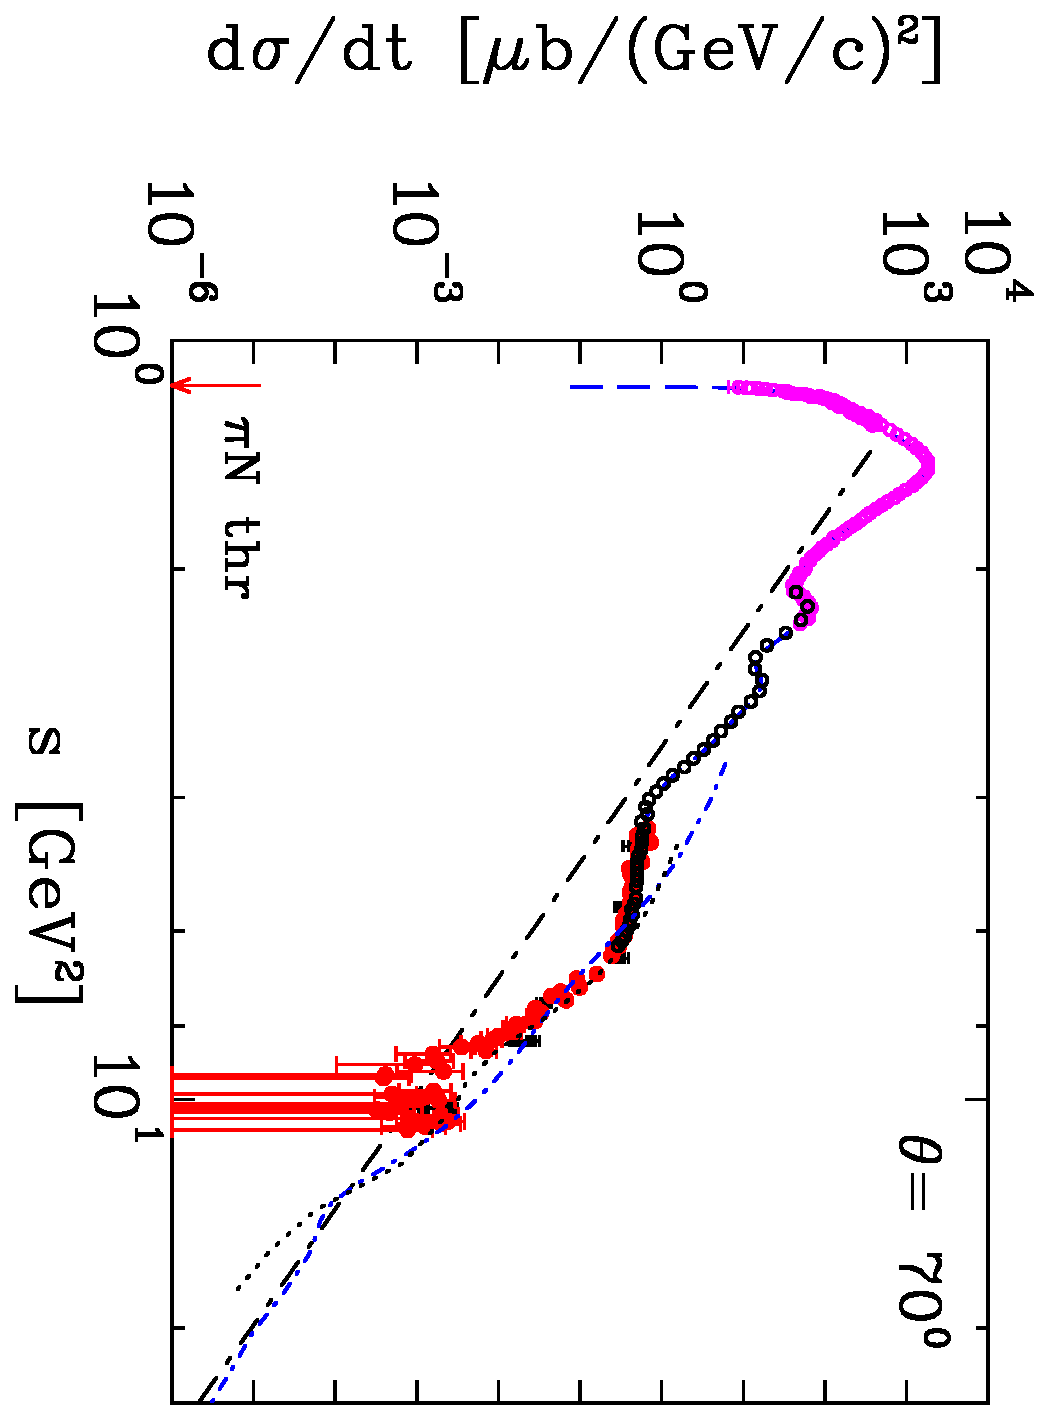
\includegraphics[height=0.4\textwidth, angle=90]{scale70.eps}}
\centerline{
        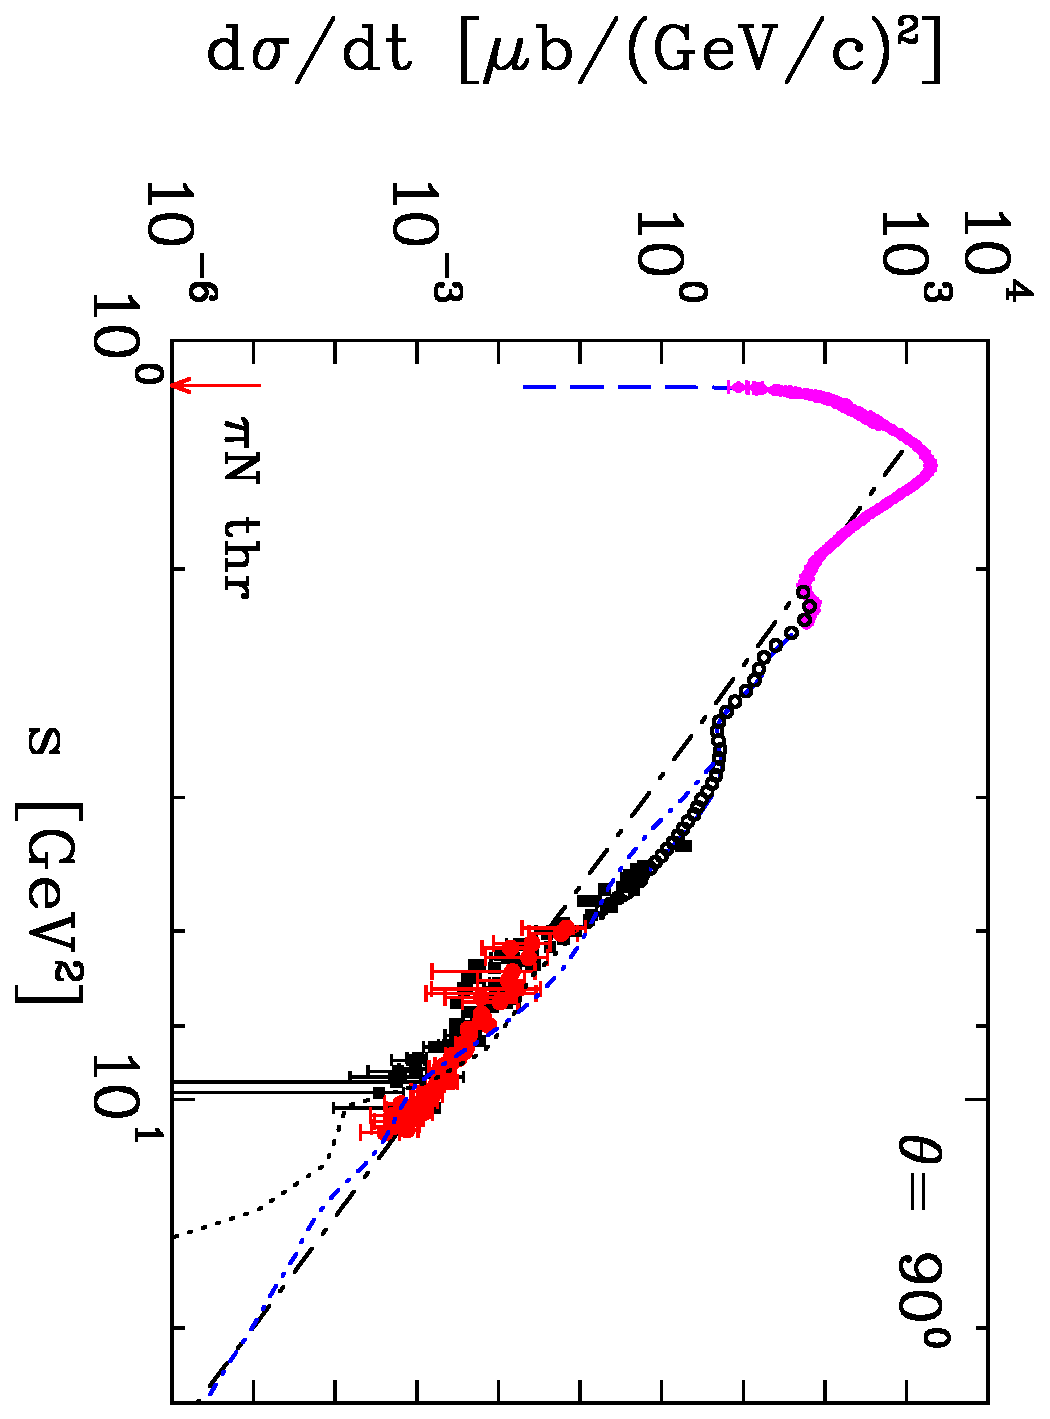
\includegraphics[height=0.4\textwidth, angle=90]{scale90.eps}\hfill
        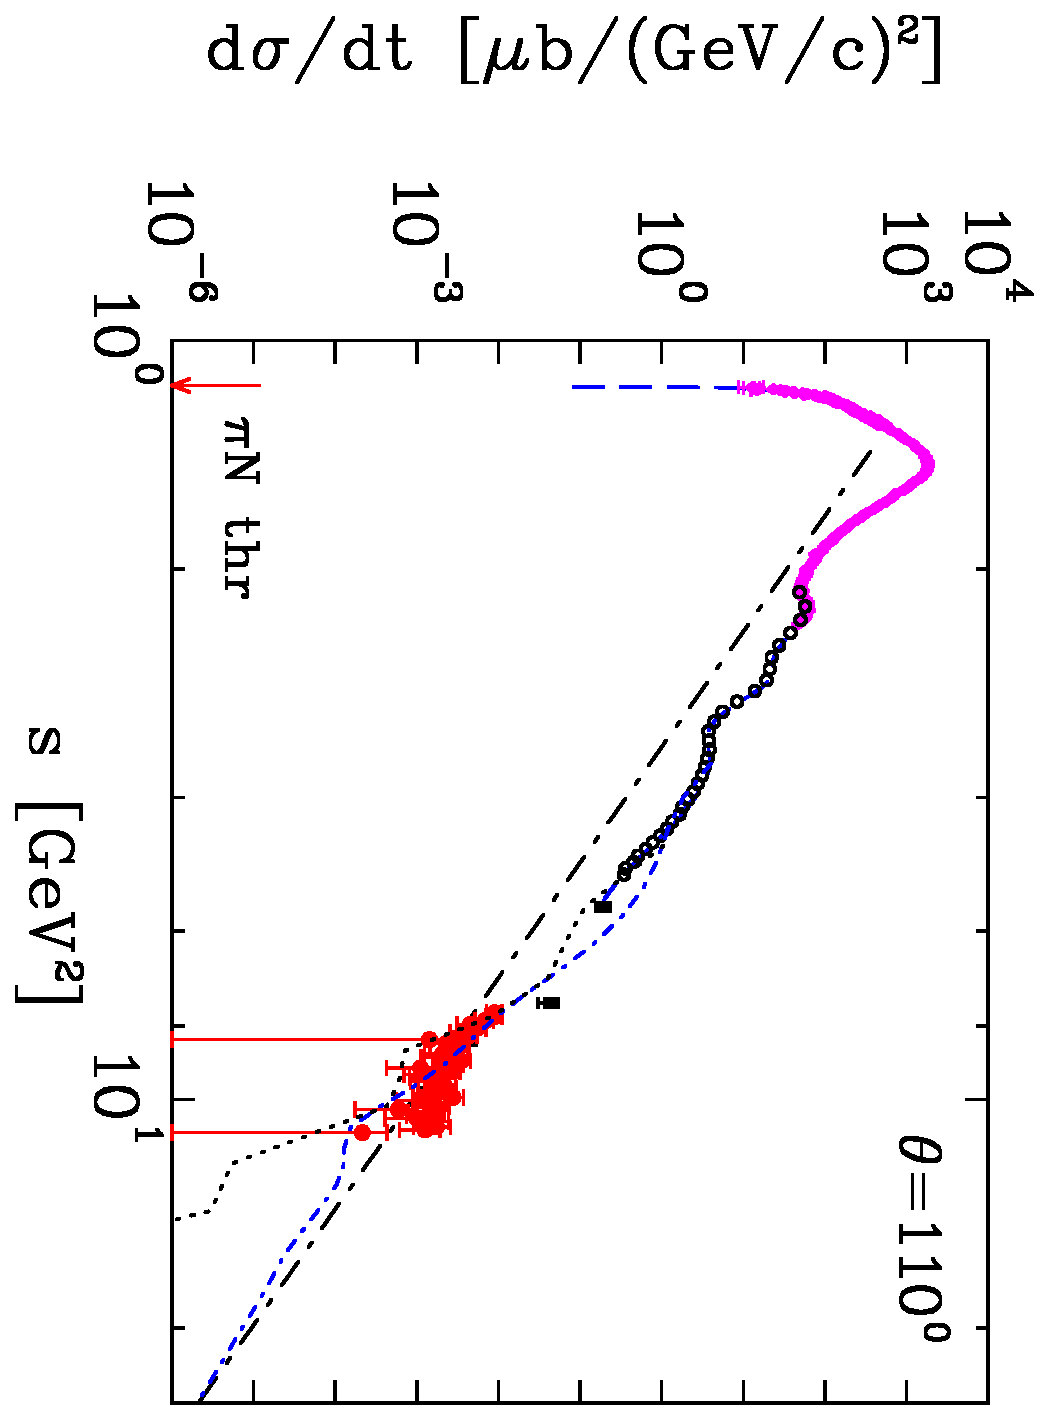
\includegraphics[height=0.4\textwidth, angle=90]{scale110.eps}}

        \caption {(Color online) Differential cross section of 
		$\gamma p\to\pi^0p$ d$\sigma$/dt(s) at 
		50$^\circ$, 70$^\circ$, 90$^\circ$, and 
		110$^\circ$ in c.m. as a function of c.m. 
		energy squared, $s$. The red filled circles are 
		results from the current analysis of the CLAS 
		Collaboration $g12$ data. The recent tagged data 
		are from CLAS $g1c$~\protect\cite{du07} (black 
		open circles) and A2 at MAMI 
		Collaboration~\protect\cite{mami} (magenta open 
		dymonds with crosses). While black open filled 
		squares are data from old bremsstrahlung
		measurements above E = 2~GeV~\protect\cite{brem}. 
		The plotted points from previously published 
		experimental data within $\Delta\theta =
		\pm$2$^\circ$ of pion c.m. production angle, 
		$\theta$.  Plotted uncertainties are statistical.  
		The blue dashed line corresponds to the SAID PWA 
		DU13 solution (no new CLAS data are in the 
		fit)~\protect\cite{du13}.  Black dot-dashed lines 
		are plotted to help guide the eye except the 
		90$^\circ$ case (see text for details). Pion 
		production threshold shown as a vertical red 
		arrow.} \label{fig:scaling}
\end{figure}
%-----------------------------------------------------

%-----------------------------------------------------
\begin{figure*}[htb!]
\centerline{
        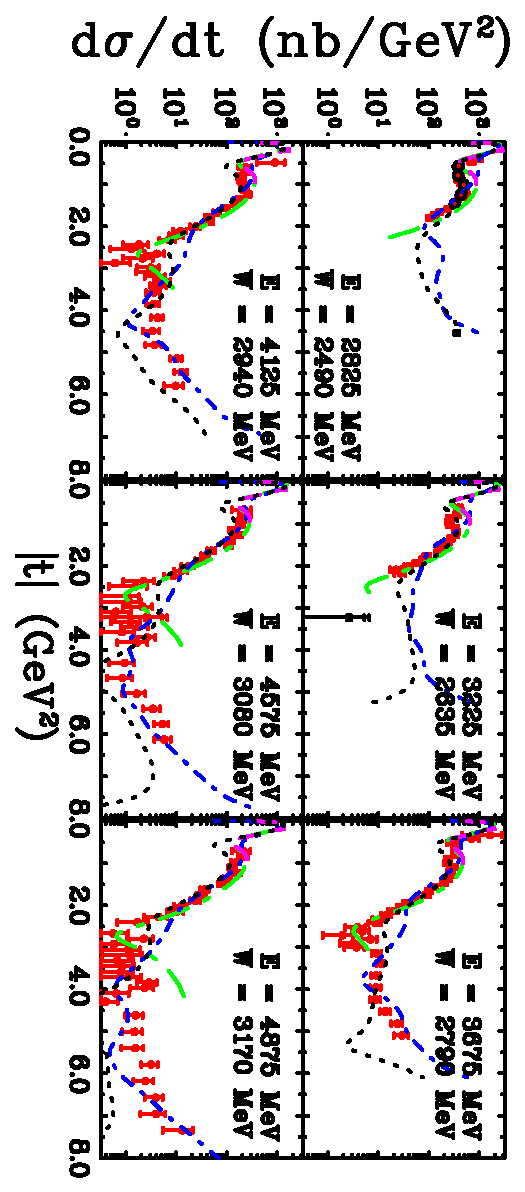
\includegraphics[width=3in, angle=90]{dsdt.eps}}

        \caption {(Color online) Samples of the $\pi^0$ 
		photoproduction cross section, $d\sigma/dt(|t|)$, 
		off the proton versus $|t|$ above "resonance" 
		regime.  Tagged experimental data are from the 
		current CLAS $g12$ (red filled circles) and CLAS 
		$g1c$~\protect\cite{du07} (black open circles). 
		The plotted points from previously published 
		bremsstrahlung experimental data above E = 
		2~GeV~\protect\cite{brem} (black filled squares) 
		are those data points within $\Delta E = \pm$3~MeV 
		of photon energy in laboratory system indicated on 
		each panel. Plotted uncertainties are statistical.  
		Regge results~\protect\cite{Goldstein,Mathieu,
		Donnachie} are given by black dotted, green 
		long dash-dotted, and black short dash-dotted
		lines, respectively.} \label{fig:t_data}
\end{figure*}
%-----------------------------------------------------

%-----------------------------------------------------
%\textbf{Scaling:}  
At high energies (above $s$ = 5.9~GeV) and large angles 
(90$^\circ$) in c.m the results are consistent with the 
$s^{-7}$ scaling expected from the constituent counting 
rule~\cite{stan}. The black dash-dotted line on 90$^\circ$ 
(Fig.~\ref{fig:scaling}) is a result of the fit of new CLAS 
$g12$ data only, performed with power function $\sim s^{-n}$, 
leading to n = 6.89$\pm$0.26.

%-----------------------------------------------------
%\textbf{Comparison to Phenomenological Models:} 
In Figs.~\ref{fig:t_data} and \ref{fig:kroll}, the 
$d\sigma/dt(|t|)$ are shown along with predictions from Regge 
pole~\cite{Goldstein,Laget,Mathieu,Donnachie} and 
handbag~\cite{Kroll} models. Two Regge models are valid up to
$|t|=1~GeV^2$~\cite{Mathieu,Donnachie} while two others are
valid up to $|t|$ maximum ($|t|\sim 9~GeV^2$ for E = 
5.425~GeV)~\cite{Goldstein,Laget}.  Meanwhile. handbag model
is good for $-0.6~\leq \cos\theta~\leq 0.6$.

Below $|t|\sim 0.6~GeV^2$ ($t$ is the squared four-momentum 
transfer), there is a small difference between different Regge 
approaches.  Overall, the Regge approximation becomes less 
relevant below E = 3~GeV (Fig.~\ref{fig:t_data}).  CLAS data 
make this statement more apparent.  Note that some small 
structures start to appear around $|t| = 0.3-0.6~GeV^2$~($\cos\theta 
= 0.6-0.8$ below E = 4~GeV.  The dip around $|t| = 0.9-1.2~GeV^2$ 
($\cos\theta = 0.2-0.4$) (moving with energy) agrees with presented 
CLAS data.  This is surprising.  There was no evidence found before 
(with the actual data) for this dip. Note that the Regge amplitudes 
imposes non negligible constraints for the "resonance" region.  Our 
data show two more visible dips above E = 4~GeV and around $|t|\sim 
3~GeV^2$ and $|t|\sim 5~GeV^2$ which are disfavor Regge model.  
That's why it's also important to study the high energy region, 
above "resonance" regime.

The Reggeon trajectories and cancellation of singularities in $|t|$ 
gives rise to zeroes in the various combinations of helicity 
amplitudes. These are seen as dips in the cross sections. Dips that 
occur for one Regge trajectory are filled in by the contributions 
from other, distinct trajectories. That is, the zeroes for the 
$\rho^0, \, \omega$ trajectories occur at different values of $|t|$ 
than those of the $b_1^0, \, h_1$ trajectories. Nevertheless, 
because the two sets have opposite naturality (parity $(-1)^J$ or 
$(-1)^{J+1}$), there are combinations of helicity amplitudes that 
will separate into "natural" and "unnatural" parity.  Those would 
have zeroes separately. Since zeroes are not observed, but dips 
are, a mechanism for producing those dips is provided by final 
state interactions which correspond to Regge cuts (for an 
alternative Regge cut model see, for instance, Ref.~\cite{Laget}). 
Those were implemented in an eikonal formalism. It was expected 
that the appropriate range of $|t|$ was roughly $0 < |t| < 
1.3~GeV^2$. Since the newly assembled data reach all $|t|$, it is 
interesting to see how the old model, for instance~\cite{Goldstein}, 
fares in an enlarged range. Remarkably, with a lowering of the 
original Pomeron strength (by eyeball), the model fits the data 
fairly well up to the $90^\circ$.  The description of the $\pi^0$ 
photoproduction cross sections at largest $|t|$ requires some
improvement of the Regge model by probably including u-channel 
exchange.

Simultaneously, Fig.~\ref{fig:kroll} shows that new CLAS data 
disesteem the handbag model for $\pi^0$ photoproduction below 
$s$ = 11~GeV$^2$.

%------------------------------------------------------
\begin{figure}[htb!]
\centerline{
        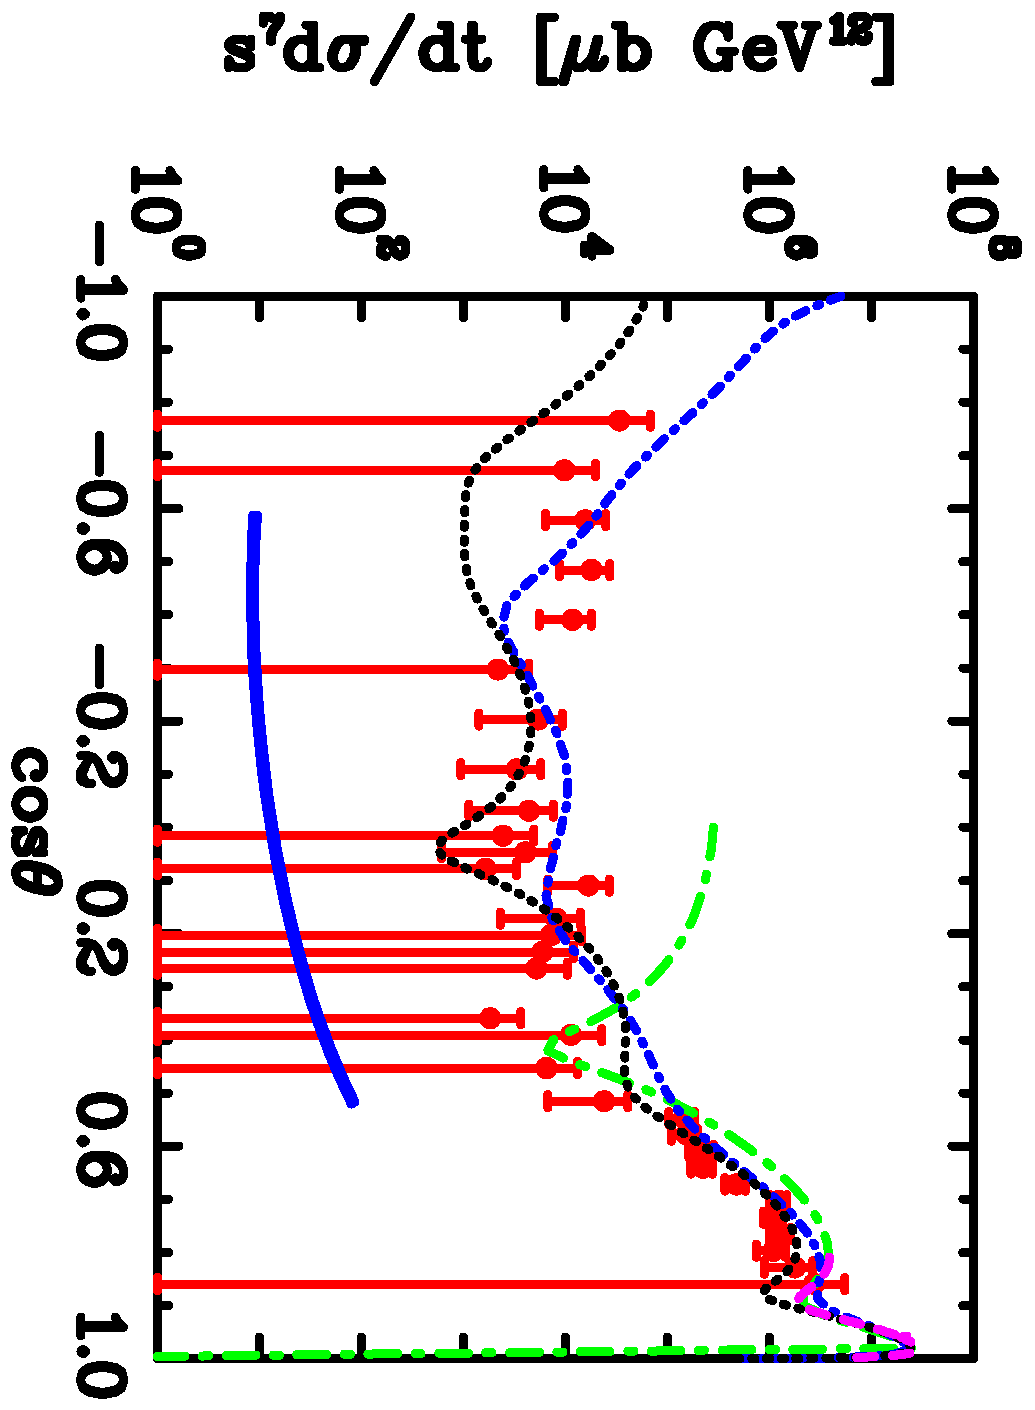
\includegraphics[width=2.5in, angle=90]{kroll.eps}}

        \caption {(Color online) Differential cross section 
		of $\pi^0$ photoproduction. CLAS experimental 
		data at $s$ = 11~GeV$^2$ are from the 
		current $g12$ experiment (red filled circles).  
		The theoretical curves a given for Regge 
		fits~\protect\cite{Goldstein,Laget,Mathieu,
                Donnachie} at $s$ = 11~GeV$^2$ (black dotted, 
		blue short dot-dashed, green long dash-dotted, 
		and black short dash-dotted lines, 
		respectively) and handbag model by 
		Kroll~\protect\textit{et 
		al.}~\protect\cite{Kroll} at $s$ = 10~GeV$^2$ 
		(blue double solid line).} 
		\label{fig:kroll}
\end{figure}
%------------------------------------------------------

%----------------------------------------------
\textbf{Conclusions:} A significant increase in the 
comprehensiveness of the database for observables in the meson 
photoproduction process is critical to reaching definitive 
knowledge about QCD-based models of the nucleon. Studies that 
cover a broad range of c.m. energy $W$ are particularly 
helpful in sorting out the phenomenology.

Through the experiments described above, an extensive and
precise data set (2030 data points) on the differential cross
section for $\pi^0$ photoproduction from the proton has been
obtained over the range of $1.81~\leq W\leq 3.33$~GeV. A novel 
approach based on the use of Dalitz decay mode was employed 
for extracting the cross sections from the experimental data.

The measurements obtained here have been compared to
existing data. The overall agreement is good, while the 
data provided here quadripleted the world bremsstrahlung 
database above E = 2~GeV, more precise than previous 
measurements, and cover the reported energies with finer 
resolution.  By comparing this new and greatly expanded data 
set to the predictions of several phenomenological models, 
the present data were found to favor the Regge pole model 
while disfavor while disfavor handbag one.  

The present set of cross sections...\\

%---------------------------------------------
\textbf{Acknowledgements:}  We thank Alexander Donnachie, 
Gary Goldstein, Peter Kroll, Jean-Marc Laget, Vincent Mathieu, 
and Anatoly Radyushkin for comments on the feasibility of our 
measurements. We would like to acknowledge the outstanding 
efforts of the staff of the Accelerator and the Physics 
Divisions at Jefferson Lab that made the experiment possible.  
This work was supported in part by the Italian Istituto 
Nazionale di Fisica Nucleare, the French Centre National de 
la Recherche Scientifique and Commissariat \`a l'Energie 
Atomique, the United Kingdom's Science and Technology 
Facilities Council (STFC), the U.S. DOE and NSF, and the 
Korea Science and Engineering Foundation. The Southeastern 
Universities Research Association (SURA) operates the Thomas 
Jefferson National Accelerator Facility for the US DOE under 
contract DEAC05--84ER40150.

%-----------------------------------------------------------
\begin{thebibliography}{99}
\bibitem{Ader} J.~P.~Ader, M.~Capdeville, and Ph.~Salin, Nucl.\ 
	Phys.\ \textbf{B3}, 407 (1967).
\bibitem{Goldstein} G.~R.~Goldstein and J.~F.~Owens~III, Phys.\ 
	Rev.\ D\ \textbf{7}, 865 (1973).
\bibitem{Laget} J.-M.~Laget, Phys.\ Rev.\ C\ \textbf{72}, 
	022202(R) (2005).
\bibitem{Mathieu} V.~Mathieu, G.~Fox, and A.~Szczepaniak, Phys.\ 
	Rev.\ D\ \textbf{92}, 074013 (2015).
\bibitem{Donnachie} A.~Donnachie and Yu.~S.~Kalashnikova, Phys.\ 
	Rev.\ C\ \textbf{93}, 025203 (2016).
\bibitem{Kroll} H.~W.~Huang and P.~Kroll, Eur.\ Phys.\ J.\ C\ 
	\textbf{17}, 423 (2000);
        H.~W.~Huang, R.~Jakob, P.~Kroll, and K.~Passek-Kumericki, 
	Eur.\ Phys.\ J.\ C\ \textbf{33}, 91 (2004);
        M.~Diehl and P.~Kroll, arXiv:1302.4604 [hep--ph].
\bibitem{HM}X.~Ji, Phys.\ Rev.\ Lett.\ \textbf{78}, 610 (1997); 
	Phys.\ Rev.\ D\ \textbf{55}, 7114 (1997); 
	A.~V.~Radyushkin, Phys.\ Lett.\ B\ \textbf{380}, 417 (1996); 
	Phys.\ Rev.\ D\ \textbf{56}, 5524 (1997); 
	M.~Diehl, T.~Feldmann, R.~Jakob, P.~Kroll, Eur.\ Phys.\ J.\ 
	C\ \textbf{8}, 409 (1999).
\bibitem{Moskov}M.~Amarian \textit{et al.} (HERMES Collaboration), 
	AIP\ Conf.\ Proc.\ \textbf{570}, 428 (2001), Proceedings 
	of the \textit{14th International Spin Physics Symposium} 
	(SPIN 2000), Osaka, Japan, Oct. 2000, edited by K.~Hatanaka, 
	T.~Nakano, K.~Imai, and H.~Ejiri.
\bibitem{brem} The Durham HEP Reaction Data Databases (UK) (Durham 
	HepData): http://durpdg.dur.ac.uk/hepdata/reac.html .
%	P.~Joss, \textit{Compilation of Photoproduction Data
%        above 1.2~GeV}, DESY-HERA 70-1, 1970.
\bibitem{PDG} K.~A.~Olive \textit{et al.} (Particle Data Group), 
	Chin.\ Phys.\ C\ \textbf{38}, 090001 (2014).
\bibitem{du07} M.~Dugger \textit{et al.} (CLAS Collaboration), 
	Phys.\ Rev.\ C\ \textbf{76}, 025211 (2007).
\bibitem{mami}M.~Fuchs \textit{et al.}, Phys.\ Lett.\ B\ 
	\textbf{368}, 20 (1996); 
	R.~Beck \textit{et al.}, Eur.\ Phys.\ J.\ A\ \textbf{28S1}, 
	173 (2006).
\bibitem{du13} M.~Dugger \textit{et al.} (CLAS Collaboration), 
	Phys.\ Rev.\ C\ \textbf{88}, 065203 (2013).
\bibitem{stan}S.~J.~Brodsky and G.~F.~de~Teramond, Phys.\ Lett.\ 
	B\ \textbf{582}, 211 (2004); 
	S.~J.~Brodsky \textit{et al.}, Phys.\ Rev.\ D\ \textbf{69}, 
	076001 (2004).
\bibitem{scaling1}
S.~J.~Brodsky  and G.~R. Farrar.
%\newblock Scaling laws at large transverse momentum.
\newblock {Phys. Rev. Lett.}, \textbf{31},1153--1156, 1973.

\bibitem{scaling2}
G.~Peter Lepage and S.~J. Brodsky.
%\newblock Exclusive processes in perturbative quantum chromodynamics.
\newblock {Phys. Rev. D}, \textbf{22},2157--2198, 1980.

\bibitem{scalingexp5}
P.~V. Landshoff and J.~C. Polkinghorne.
%\newblock pp elastic scattering at large momentum transfer.
\newblock {Physics Letters B}, \textbf{44}(3),293 -- 295, 1973.

\bibitem{scalingexp7}
R.~L. Anderson et~al.
%\newblock Comparison of 20 exclusive reactions at large t.
\newblock {Phys. Rev. D}, \textbf{49}, 1994.

\bibitem{scalingexp2}
W.~Chen et~al.
%\newblock Measurement of the differential cross section for the reaction
%$\ensuremath{\gamma}n\ensuremath{\rightarrow}{\ensuremath{\pi}}^{-}p$ from
%deuterium.
\newblock {Phys. Rev. Lett.}, \textbf{103},012301, 2009.

\bibitem{scalingexp3}
L.~Y. Zhu et~al.
%\newblock Cross-section measurement of charged-pion photoproduction from
%hydrogen and deuterium.
\newblock {Phys. Rev. Lett.}, \textbf{91},022003, 2003.

\bibitem{scalingexp4}
R.~A. Schumacher and M.~M. Sargsian.
%\newblock Scaling and resonances in elementary ${K}^{+}\ensuremath{\Lambda}$
%photoproduction.
\newblock {Phys. Rev. C}, \textbf{83}, 2011.

\bibitem{scalingexp6}
R.~L. Anderson et~al.
%\newblock Measurements of exclusive photoproduction processes at large values
%of $t$ and $u$ from 4 to 7.5 gev.
\newblock {Phys. Rev. D}, \textbf{14},679--697, 1976.

\bibitem{scalingexp8}
J.~Napolitano et~al.
%\newblock Measurement of the differential cross section for the reaction
%$^{2}\mathrm{H}(\ensuremath{\gamma},p)n$ at high photon energies and
%${\ensuremath{\theta}}_{\mathrm{c}.\mathrm{m}.}=90\ifmmode^\circ\else\textdegree\fi{}$.
\newblock {Phys. Rev. Lett.}, \textbf{61},2530--2533, 1988.

\bibitem{scalingexp9}
J.~E. Belz et~al.
%\newblock Two-body photodisintegration of the deuteron up to 2.8 gev.
\newblock {Phys. Rev. Lett.}, \textbf{74},646--649, 1995.

\bibitem{scalingexp10}
C.~Bochna et~al.
%\newblock Measurements of deuteron photodisintegration up to 4.0 gev.
\newblock {Phys. Rev. Lett.}, \textbf{81},4576--4579, 1998.

\bibitem{scalingexp11}
E.~C. Schulte and others.
%\newblock Measurement of the high energy two-body deuteron photodisintegration
%differential cross section.
\newblock {Phys. Rev. Lett.}, \textbf{87}, 2001.
\bibitem{g12note}
Z.~Akbar et~al.
\newblock {g12 Analysis Procedures, Statistics and Systematics}.
\newblock Technical report, \texttt{CLAS} Technical Note, 2016.

\bibitem{mkthesis}
M.C.Kunkel.
\newblock {\em {Photoproduction of $\pi^{0}$ on hydrogen with CLAS from 1.1 GeV
		- 5.45 GeV using $\lowercase{e}^{+}\lowercase{e}^{-}\gamma$ decay}}.
\newblock {PhD} dissertation.
\newblock \url{https://www.jlab.org/Hall-B/general/thesis/Kunkel_thesis.pdf}.	
%\bibitem{Arndt90a}R.~A.~Arndt \textit{et al.}, Phys.~Rev. C \textbf {42}, 
%	1853 (1990).
%\bibitem{Walker}R.~L.~Walker, Phys.~Rev. \textbf {182}, 1729 (1969).
%\bibitem{CGLN} G.~F.~Chew, M.~L.~Goldberger, F.~E.~Low, and Y.~Nambu, 
%	Phys.\ Rev.\ \textbf{106}, 1345 (1957).
%\bibitem{Watson52}K.~M.~Watson, Phys.~Rev. \textbf{85}, 853 (1952).
%\bibitem{Rosenfeld}R.~G.~Moorhouse, H.~Oberlack, and A.~H.~Rosenfeld, 
%	Phys.\ Rev.\ D\ \textbf{9}, 1 (1974).
%\bibitem{graal} O.~Bartalini \textit{et al.} (GRAAL Collaboration), 
%	Eur.\ Phys.\ J.\ A\ \textbf{26}, 399 (2005).
%\bibitem{leps} M.~Sumihama \textit{et al.} (LEPS Collaboration), Phys.\ 
%	Lett.\ B\ \textbf{657}, 32 (2007).
%\bibitem{cbelsa} V.~Crede \textit{et al.} (CB-ELSA Collaboration), 
%	Phys.\ Rev.\ C\ \textbf{84}, 055203 (2011);
%	Bartholomy \textit{et al.} (CB-ELSA Collaboration), Phys.\ Rev.\ 
%	Lett.\ \textbf{94}, 012003 (2005).
%\bibitem{maid} The MAID analyses are available through the Mainz website:
%	http://wwwkph.kph.uni-mainz.de/MAID/. See also D.~Drechsel, 
%	S.S.~Kamalov, and L.~Tiator, Eur.\ Phys.\ J.\ A\ \textbf{34}, 69 
%	(2007).
%\bibitem{said} W.~J.~Briscoe, I.~I.~Strakovsky, and R.~L.~Workman, 
%	Institute of Nuclear Studies of The George Washington University 
%	Database: 
%	http://gwdac.phys.gwu.edu/analysis/pranalysis.html .
%\bibitem{sp06} R.~A.~Arndt, W.~J.~Briscoe, I.~I.~Strakovsky, and 
%	R.~L.~Workman, Phys.\ Rev.\ C\ \textbf{74}, 045205 (2006).
%\bibitem{hallC}\textit{Wide angle exclusive photoproduction of $\pi^0$
%	mesons}, Spokespersons: D.~Dutta, H.~Gao, S.~Sirca, M.~Amaryan,
%	M.~Kunkel, and I.~Strakovsky (RCS and NPS Collaborations), JLab 
%	Proposal E12--14--005, Newport News, VA, USA, 2014.
%\bibitem{an71}R.L.~Anderson \textit{et al.}, Phys.\ Rev.\ D\ \textbf{4}, 
%	1937 (1971).
%\bibitem{ba74}B.~Barish \textit{et al.}, Phys.\ Rev.\ D\ \ D\ \textbf{9}, 
%	566, (1974).
%\bibitem{os72}A.M.~Osborne \textit{et al.}, Phys.\ Rev.\ Lett.\ \textbf{29}, 
%	1621, (1972).
%\bibitem{br73}W.~Braunschweig \textit{et al.}, Nucl.\ Phys.\ \textbf{B51} 
%	157 (1973).
\end{thebibliography}
%---------------------------------------------------------------------
\end{document}
